\section{The engine, change by change}\label{sec:engine}

Each item names what stock did, what the fork does, the knob that restores the old path where there is one, and the
measured effect at the time it was added (the models and thread counts differ because the suite grew;
Figure~\ref{fig:progress} has the common view; the SMA launch is on its 1.071\,M-cell mesh up to cg18 and on its
0.871\,M-cell mesh in the items of cg29, Table~\ref{tab:models}). All items are bit-identical to stock on the six models, the
cylindrical multigrid example and the special cases of Section~\ref{sec:policy} unless stated, for clang builds
(Section~\ref{sec:contract}). The on/off knobs named below act when set to any value other than empty or \code{0}
(patch 0006; \code{OPENEMS\_FUSED=0}, \code{OPENEMS\_BALANCE=0} and \code{OPENEMS\_QOS} keep their meaning, the
switches that cg29 adds with \code{=0} act, like \code{OPENEMS\_FUSED=0}, on any non-empty value that \code{atoi}
reads as 0 (so \code{off} too), and an empty value of any of the fork's variables counts as unset). Class and file names are
those of v0.37.0 and of the gpu-engine base 7bb294f that the patches apply to (Section~\ref{sec:baseline}); upstream
master reorganised these classes on 2026-11-02, and the patches do not apply to it as they are. A companion document in
the repository (Section~\ref{sec:repro}), \code{paper/code\_notes.md}, written from the diffs by an AI review agent,
gives file names, line counts and code fragments for every item of patches 0001--0006 (cg18); it does not cover the
later patches, whose commit messages describe them: the Metal diamond engine of patches 0007--0016 is in
Section~\ref{sec:gpu}, the CPU items of patches 0017--0027 (cg29) in Section~\ref{sec:cg29}, patches 0028--0039
(cg31) in Section~\ref{sec:cg31}. This section keeps to the
mechanisms.

\paragraph{Memory layout, for reference.} The SSE engines store each field as a 4-D array of \code{f4vector}s in
I-J-K-N order (component stride 1, z-vector stride 3), so one $(x,y,z_v)$ holds the three components of four cells;
cell $z$ sits in lane $z/n_v$ of z-vector $z \bmod n_v$ with $n_v=\lceil N_z/4\rceil$, and the z extent is padded to
$4n_v$. A cell costs 12\,B per field. The compressed operator index needs one 32-bit entry per z-vector, 1\,B per
cell. Up to cg28 it was allocated with one entry per cell ($N_x N_y N_z$), of which only the first $n_v$ of each z-row
were used, so with 128-B cache lines the engine streamed up to 4\,B of index per cell, all of it when $N_z \le 42$;
cg29 allocates it per z-vector (Section~\ref{sec:cg29}). The byte counts below give the compact 1\,B and, where it
mattered up to cg28, the index as allocated. The Metal diamond engine keeps the same \code{f4vector} fields in N-I-J-K
order (component outermost) in memory shared with the GPU, so probes, dumps and the CPU extensions read the same arrays
(Section~\ref{sec:gpu}).

\subsection{Barriers and the hook plan (snapshot A)}
Stock \code{Engine\_Multithread} separates the pieces of a time step with a \code{boost::barrier} (mutex and
condition variable): voltage update, barrier, then \emph{for every extension} each of the six hooks followed by a
barrier, whether or not the extension implements it; $2+6N$ barriers per step for $N$ extensions, 50 on the patch
model (one excitation, six Mur faces, and the lumped-RLC extension of the port's feed resistor, which stock keeps with
no active cell because its \code{BuildExtension} returns true), each a kernel round trip. Thread 0 also incremented
the time-step counter after the last hook with no barrier before the other threads' next step.

The fork replaces the barrier with a spin barrier (\code{tools/spin\_barrier.h}): an atomic arrival counter and a
generation number; the last arrival bumps the generation (and, when asked, the time-step counter, which removes the
race), waiters spin on the generation with a CPU pause for up to 50\,$\mu$s (\code{OPENEMS\_BARRIER\_SPIN\_US})
and only then park on a condition variable. Every extension now declares which hooks it uses
(\code{GetUsedHooks()}, a bit mask), and a \emph{hook plan} is built per engine: extensions that do not declare a hook
group are not called at all; pre- and post-hooks of all declaring extensions share one barrier at the end of their
group (they only read engine fields, by contract; the UPML, whose pre/post hooks swap field and flux, declares
\code{PREPOST\_WRITES\_FIELDS} and gets its barriers back); the apply hooks keep one barrier per extension because
they write fields in priority order. Extensions that declare nothing keep the stock behaviour. Unfused, the count
becomes $2 + [\text{any pre-V}] + [\text{any post-V}] + \#\text{apply-V} + [\text{any pre-I}] + [\text{any post-I}] +
\#\text{apply-I}$: 12 on the patch model with the current declarations (one apply barrier each for the lumped-RLC
extension, the six Mur faces and the excitation, the shared pre- and post-voltage barriers and the two update
barriers); 18 at snapshot A, where the lumped-RLC extension still declared nothing, and 13 until patch 0005, where the
excitation also declared the apply-current group. With the fused sweep below it is exactly 2, and with the neighbour
flags of cg29, when every extension allows them, none: the threads then meet only at the start and the end of a run of
steps (Section~\ref{sec:cg29}). The plan is rebuilt
whenever the extension list changes; the first version was built once, before the cylindrical multigrid registered
its child engines, and was wrong on that example only, which is why the check suite runs it.
Patch tutorial 277 to 502\,\MC, notch tutorial 318 to 573, patch x5 1\,041 to 1\,151 (the load sampler failed on that
8-thread run; the 10-thread run, at 56\,\% other load, gave 1\,121), notch x3 845 to 902.

\subsection{The inner loop (AB)}
\code{Engine\_SSE\_Compressed::UpdateVoltages} located every operand through the array library's subscript
operators and, because Apple clang gives every store through the \code{f4vector} union the alias type of \code{char}
(the TBAA type `omnipotent char', which may alias any object), reloaded strides and coefficient pointers after every
store: 94 instructions per vector update (the three components of one z-vector), 44 of them loads, of which 21 load
vectors (95 and 44 for the currents). \code{UpdateVoltages\_IJKN} / \code{UpdateCurrents\_IJKN} walk the I-J-K-N
layout with all invariants in local variables and \code{\_\_restrict} pointers (the three components of a z-vector
at \code{vz[0..2]}, the next z-vector at \code{+3}, the x and y neighbours at constant offsets, the z wrap-around
with a lane shift) and store each component once: 44 instructions at snapshot AB (from the project log); 41 with 16
loads in cg18, which also reads the packed tables of cg13 (42 and 15 for the currents). The stock and
cg18 counts, taken in the copy of each loop that runs, are in
\code{results/kernel\_loop\_instructions\_2026-11-03.txt}. Per component
stock computes $v \leftarrow v\cdot vv$ then $v \leftarrow v + vi\cdot t$ with $t=(c_1-c_2)-c_3+c_4$; the new code
computes $a = v\cdot k_0$, $v = a + k_1 t$ with the identical $t$, and with clang's default contraction both forms
become a rounded product followed by one fused multiply-add, so the bit patterns agree. This identity was verified by
comparison (and against the Metal mirror of the same loop), not forced in the source; GCC contracts the two forms
differently (Section~\ref{sec:contract}). Traffic is unchanged by this item (37\,B per cell per update with a compact
index, 40\,B with the index as allocated). Patch tutorial 502 to 579, notch tutorial 573 to 668, patch x5 1\,151 to
1\,258. The stock baseline is the default clang build. Upstream's FAQ~\cite{biergaizi29} asks macOS users to build
openEMS with GCC because clang's code for the SSE engine is slow. In the standalone kernel
(\code{scripts/kernel/kb\_idx.cpp}) GCC~16 does not reload the strides and pointers: its stock loop has 80--82
instructions and 29 loads, 7 of them reloads of spilled registers (same instruction-count file). At one thread, on
three grids outside the valley of Section~\ref{sec:valley} (\code{results/kernel\_gcc\_vs\_clang\_2026-11-03.txt}),
it runs the stock loop 1.16--1.39$\times$ faster than Apple clang, while the rewritten loop runs at about the same
speed with both: the rewrite's one-thread gain in the kernel is 1.26--1.47$\times$ with both loops built by GCC and
1.74--1.80$\times$ with both built by clang. A GCC build of openEMS itself was not made, so whole runs with GCC were
not measured, and the factors of this paper are against stock built with Apple clang, the default compiler on macOS.

\subsection{Work distribution and the automatic thread count (C, refined up to cg8)}
Stock gives every thread a fixed x-slab of equal width, and \code{numThreads=0} (the default) starts with one thread
and adds one at every progress report, about every 4\,s, until the reported speed drops: a 1$\to$N ramp. In
Table~\ref{tab:step1} the default is 37--41\,\% slower than the best fixed count on the two large models (15--20\,s
runs), 22\,\% on the 17.5\,s notch tutorial run and 8\,\% on the 4\,s patch tutorial. On a 4P+6E machine equal slabs
are wrong twice over: an E core takes longer, and the first and last slabs hold the PML.

The fork does three things. In the unfused path, threads take x-lines from per-thread atomic counters and steal
from the other threads' ranges when their own is done (the order of lines within one update is irrelevant: the
voltage update reads only currents and vice versa, and each line is written by exactly one thread). In the fused
path (next item) threads own contiguous slabs and \code{BalanceSlabs()} moves the slab boundaries after every
\code{IterateTS} call once 20\,ms of sweeps have accumulated, to equal cumulative cost per thread from the measured
busy time per line (\code{OPENEMS\_BALANCE=0} turns it off). And the automatic thread count is chosen by measurement
on the running simulation: starting at the P-core count (\code{hw.perflevel0.physicalcpu} on Apple, half the available
hardware threads elsewhere), \code{IterateTS} runs in pieces of an eighth of a 150\,ms window
(\code{OPENEMS\_TUNE\_WINDOW\_MS}) with balancing between pieces; each candidate count is timed for one window after a
settling time of 0.4 windows; the search goes P, P+2, P+4, \ldots\ (stopping once a count falls below 85\,\% of the
best), then P$-$2, then $\pm1$ around the best, and prints the result. Every candidate is clamped to the number of
x-lines (patch 0005 clamped only the larger ones; patch 0006 also clamps P$-$2 and the start). The tuner and its
150\,ms windows date from C; slab balancing followed right after ABCDEG and is in every cg snapshot; the window/8
pieces and the search order came with cg7 and cg8. Speed is not monotonic in the thread count (notch x3 at cg8:
4:1791, 5:1564, 6:1800, 7:1919, 8:2022, 9:1901\,\MC; from the project log, not in \code{results/}), hence the coarse
step and the refinement.
The search needs about 1.5\,s and costs short benches 15--25\,\% (both from the project log); at cg14 it picked 4 for
models up to a few hundred thousand cells and 7--8 above a million (Table~\ref{tab:final}). With the neighbour flags
(a development build of cg29) it picked 9--10 threads in most runs on the GCPW line and the SMA launch at their real
run lengths. A cache of the chosen count per model (second review, item 3) and a 50\,ms window were measured for cg29
and gained nothing at those run lengths (Section~\ref{sec:rejected}). The cylindrical multigrid engine keeps the stock
ramp, with its inner engine pinned to one thread.

\subsection{Mur and UPML on vectors (D; Mur line hooks rebuilt in cg4)}
The Mur absorbing boundary~\cite{mur1981} and the uniaxial PML~\cite{berenger1994} extensions were written against
the scalar field interface: per face cell, \code{GetVolt}/\code{SetVolt} computes a 4-D subscript with a division and
a modulo for every access. The Mur fast path precomputes the float index of every face cell once and checks that the
offsets to the two components and to the shifted line are the same constants for all cells (otherwise the template
path stays); its three hooks are then the template's three expressions on the same operands. The UPML vector path,
for PML boxes that span the whole z range (only then does every \code{f4vector} belong entirely to the PML), copies
the six per-cell coefficient arrays and the two flux arrays into vector order and runs the update per $(x,y)$ row of
$3n_v$ vectors with a lane mask for the padding, splitting rows rather than x-lines over threads (a slab of 8 lines
would otherwise occupy at most 8 threads). The vector form $p=-(c_{\text{fo}}\cdot F)$, $f = c\cdot E + p$ pins the
contraction to what clang emitted for the scalar line (GCC fuses the other product, Section~\ref{sec:contract}).
Mur's \emph{line} hooks for the fused sweep (E) were then rebuilt in cg4: the face cells of each x-line in memory
order, the four lanes of one z-vector of an x- or y-face (cells $z, z+n_v, z+2n_v, z+3n_v$) as one vector with
lane-wise coefficients, the rest scalar. Patch tutorial 1\,519 to 1\,810, patch x5 1\,454 to 1\,602 (cg2 to cg6,
4 threads).

\subsection{The fused E/H sweep (E)}\label{sec:fused}
A time step is one pass over the voltages followed by one pass over the currents; on a model larger than the cache
every field array is streamed from DRAM twice per step, 74\,B per cell (12\,B read and 12\,B written for the updated
field, 12\,B read for the other, 1\,B of compact index, per update; 80\,B with the index as allocated). The fork
fuses the two passes. $V(x)$ reads $I(x)$ and $I(x-1)$; $I(x)$ reads $V(x)$ and $V(x+1)$. Once the voltages and
voltage hooks of x-line block $[x_0,x_1)$ are final, the currents of lines $x_0-1 \ldots x_1-2$ have all their
operands final and their old values are needed by no voltage of this step, so each thread runs, per block of its slab:
\begin{lstlisting}
RunLineHooks(PRE_VOLT, x0, x1);  UpdateVoltages(x0, x1-x0);
RunLineHooks(POST_VOLT, x0, x1); RunLineHooks(APPLY_VOLT, x0, x1);
FusedCurrents(x0==start ? x0 : x0-1, x1-1);   // pre-I hooks, I, post-I, apply-I of the line behind
...                                            // after the slab:
barrier();  if (start>0) FusedCurrents(start-1, start);   // the line before the slab, now that the neighbour's V is final
barrier(numTS++);
\end{lstlisting}
The currents of a line are computed while its voltages and the neighbouring currents are still in L1/L2, so both
fields stream once: 49\,B per cell (52\,B with the index as allocated up to cg28), and two barriers per step (neighbour
flags since cg29, Section~\ref{sec:cg29}). For this to be
legal every extension that touches fields during the step needs per-line hooks (\code{*Lines(x0,x1)}) besides the
whole-grid ones, touching only its own lines (an x-face Mur line that reads the next line declares it as
\emph{coupled}, and the two are always in one block); the excitation and the lumped RLC sort their entries by x-line
once and run their unchanged bodies on the entries of a block (up to cg28 the RLC's per-step container rotation was
done by whichever thread arrived first, under a time-step stamp; cg29 takes the three slots from the time step). Mur,
UPML, excitation, RLC, since cg12 the Drude/Lorentz extension, which also carries the conducting sheets, and since
cg29 the Debye extension and the steady-state detection have line hooks, and since cg31 the cylinder extension of
cylindrical meshes closed in alpha (Section~\ref{sec:cg31cyl}). Any extension without them (Debye materials
from patch 0005 to cg28, the cylinder extension up to cg29, the cylindrical multigrid,
TFSF, the steady-state detection up to cg28, the \code{Absorbing\_BC} extension) puts the whole run on the unfused
plan, and a verbose message names it (once per level engine of a cylindrical multigrid since patch 0006). The fused
sweep also needs the packed coefficient tables of cg13 (or, since cg29, the geometry tables of
Section~\ref{sec:cg29}); when their allocation fails, the engine says that the fused sweep is off
because there are no packed tables (patch 0006). The fused sweep never calls the current-line hooks for the last
x-line (documented in \code{engine\_extension.h}; no engine updates currents there). \code{OPENEMS\_FUSED=0} restores
two passes. Notch x3 1\,153 to 1\,916\,\MC\ in the same build, patch x5 1\,348 to 1\,559 (from the project log; not in
\code{results/}); tutorials unchanged (they fit in the cache). A standalone kernel of the same shape, but with a
compact 1-B index (\code{scripts/kernel/kb\_idx.cpp}), reaches 1\,932\,\MC\ on 4 threads (95\,GB/s at 49\,B per cell,
read:write 1:1), and one independent sub-grid per thread (\code{kb\_tb.cpp}) 2\,273 on 6: those are the ceilings (from
the project log; the kernel output is not in \code{results/}). The remaining gap on patch x5 at 8 threads (20--25\,\%,
project log) is P/E imbalance at the two barriers while macOS migrates threads and other sessions load the machine;
cg29 measured the wait (at 8 threads 24--27\,\% of the time at the two barriers, \code{OPENEMS\_FUSED\_STAT=1}) and
replaces the barriers by neighbour flags (Section~\ref{sec:cg29}). Wider blocks (\code{OPENEMS\_FUSED\_BLOCK}) lose
the L2 reuse and were measured slower (Section~\ref{sec:rejected}).

\subsection{The allocation-placement valley and staggered allocations (cg10)}\label{sec:valley}
At 4 threads the two real boards had gained only 1.4--1.7$\times$ from everything above (SMA 320 to 436\,\MC, GCPW
302 to 505 with the stagger below switched off), while the tutorials had gained 4.5--6.5$\times$ at their best thread
counts. A one-thread sweep of a PEC box with a dielectric slab over its size (Figure~\ref{fig:cache},
\code{results/cache\_valley\_2026-11-01.txt}) shows why: without the stagger, boxes of 200\,000 to 338\,000 cells ran
at 246.8--249.5\,\MC, about 3.6$\times$ slower than those of 162\,000 and 392\,000 cells (891.7 and 890.7). The
valley holds the models whose field arrays are 2--4\,MiB each, about 0.175--0.35 million cells at 12\,B per cell and
array ($N_z$ a multiple of 4; 4.2--8.4\,MB of fields): on cg18 without the stagger, 176\,720 to 338\,000
cells are slow, 172\,980 and 348\,480 fast (\code{results/cache\_valley\_placement\_2026-11-03.txt}, section 3).
Stock v0.37.0 has the same valley, 2.1--2.2$\times$ deep, at about half the fork's speed outside it
(\code{results/cache\_valley\_stock\_2026-11-03.txt}).

The trigger is where the allocator puts the two arrays. macOS~27.0.1's libmalloc places two consecutive
\code{posix\_memalign} blocks of equal size 4\,MiB + 16\,KiB apart at every tested size from just above 2\,MiB to
3\,000\,000\,B, exactly 4\,MiB apart at 4\,181\,760\,B and 4\,MiB, 8\,MiB + 16\,KiB apart from just above 4\,MiB to
8\,000\,000\,B, and the second about 6\,MiB below the first from 1.94 to 2\,MiB (section 1 of the placement file).
The slow sizes fall in the range placed 4\,MiB + 16\,KiB apart (the test has no size between 3\,000\,000 and
4\,181\,760\,B, where the arrays of the 338\,000-cell box lie); 348\,480 cells (4\,181\,760\,B per array, exactly
4\,MiB apart) are already fast. All these distances are multiples of 16\,KiB, the fast ones too, so 16\,KiB set aliasing
alone does not explain the valley; the hardware mechanism was not identified. In the standalone kernel at
$110\times110\times20$ (section 2), moving the current array by 512\,B or more, 16 and 32\,KiB included, removes the
slowdown (stock loop 210--211 to 455--464\,\MC, rewritten loop 233--234 to 779--819), and 256\,B removes part of it.
The project log of 2026-10-29 had 16 and 32\,KB offsets failing, which was then read as L1 set aliasing; at this
shape that does not reproduce.

The fix is in the array allocator (\code{tools/arraylib/impl/allocator.h}, not platform-specific): every allocation
of 256\,KiB or more with an alignment of at most 256\,B is made $256 + (2560\,k \bmod 16128)$ bytes larger and the
array starts that far into it, $k = 0, 1, \ldots$ counting such allocations in the process (63 distinct multiples of
256\,B, so any alignment up to 256\,B is kept); the base pointer is stored in the word before the array, where the
free path finds it. \code{OPENEMS\_NO\_STAGGER=1} turns the stagger off. Outside the valley it changes nothing
measurable (cg18, finer sweep: 867.7--899.7\,\MC\ with it at every size, 864.9--890.5 without it outside the
valley). It is applied on every platform, but the valley was seen only with macOS~27.0.1's allocator on the M5;
other allocators place large blocks differently, so the size window, and whether there is one, depends on the
platform. The allocator is a header, so this is an ABI change for code compiled against the old one
(Section~\ref{sec:reviewfixes}). GCPW at 4 threads 505 (stagger off) to 881\,\MC\ in one session, 868 in another. The
same snapshot fixed a crash of \code{--disable-dumps} at the end of runs with frequency-domain dumps (post-processing
of fields that were never allocated).

\begin{figure}[htbp]\centering
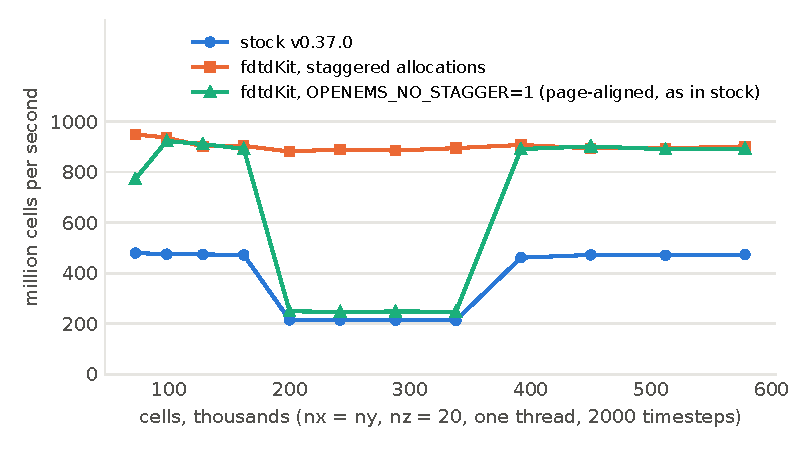
\includegraphics[width=0.7\textwidth]{fig_cache}
\caption{The allocation-placement valley on one thread: PEC box with $N_z=20$, 2\,000 steps. \mbox{fdtdKit}: the
installed cg16 build on 2026-11-01, with staggered allocations and with \code{OPENEMS\_NO\_STAGGER=1}, which leaves
the field arrays page-aligned as in stock (\code{results/cache\_valley\_2026-11-01.txt}; the low no-stagger point at
72\,000 cells is one run that was not re-measured). Stock v0.37.0: measured on 2026-11-03
(\code{results/cache\_valley\_stock\_2026-11-03.txt}).}\label{fig:cache}
\end{figure}

\subsection{PML slabs that do not span z: a scalar-SSE path and compressed tables (cg11, cg14)}
The SMA launch did not gain from the stagger. Its PML is a z-only slab at the top (13\,\% of the cells) and the UPML
vector path requires a full-z box, so those cells ran the original template: 202\,\MC\ single thread, 654 with the PML
swapped for Mur. The fork adds a scalar-SSE path for any PML box that is not a full-z slab: per local $z$ the float
offset inside an $(x,y)$ row of vectors is tabulated once ($12(z \bmod n_v) + z/n_v$), the hooks iterate rows,
components and $z$ with contiguous flux and coefficient rows, and the expression is literally the template's
($f = vv\cdot V - vv_{\text{fo}}\cdot\text{flux}$, then the swap), so the compiler contracts it the same way; each
cell-component touches only its own $V$ and flux, so the loop order does not change values. With line hooks the fused
sweep now covers the slab. SMA single thread 202 to 405, 4 threads 436 to 737, 8 threads 951 (cg29 runs this path four
y-rows at a time, Section~\ref{sec:cg29}). Of the test models only
the SMA launch, with its top z slab, takes this path. A notch tutorial run with \code{PML\_8} requested on all six
faces (\code{results/notch\_s1\_n8000\_pml6.txt}) does not: on its 14 z lines openEMS resets the z PML to PEC, and the
four x and y slabs span the whole z range. The 69\,500 distinct
operators of the SMA model cost only about 11\,\% (standalone kernel with 70\,000 operators; from the project log).
cg14 then lets the hooks read a table of distinct coefficient sets (24\,B scalar or 96\,B vector entries, a few
hundred of them: the PML profile times the materials) through a 4-B index, instead of the six per-cell coefficient
arrays (72\,B per cell). The index is per cell-component on the scalar-SSE path and per z-vector component (four
cells) on the vector path. The operator extension keeps its arrays, as in stock, and the vector path frees its own
vector copies of them, so the gain is in traffic, not in memory: with the index (and, on the vector path, the vector
copies of the flux) a PML cell holds more memory than in stock. \code{OPENEMS\_NO\_PML\_TABLE=1} keeps the hooks on
the per-cell arrays. Bandwidth-side only: SMA 4 threads 1\,137 to 1\,241, notch x3 8 threads 2\,022 to 2\,099; single
thread unchanged.

\subsection{Line hooks for the dispersive extension (cg12)}
The optimisation review of the branch found the real GCPW problem: every lossy board uses \code{AddConductingSheet},
whose engine extension (\code{Engine\_Ext\_LorentzMaterial} on \code{Engine\_Ext\_Dispersive}) implemented only the
non-threaded hooks, so the multithreaded engine ran them on thread 0 through \code{GetVolt}/\code{SetVolt}, declared
nothing (19 barriers per step on that model at cg11) and kept the whole run on the unfused plan. The fork gives the
dispersive extensions line hooks: the auxiliary-differential-equation positions of every order are stable-sorted by
x, the float index of each component is precomputed, the per-position arithmetic is the template's (apply:
$v \leftarrow v - \text{ade}$; Lorentz pre-hooks: the template's three statements), and the extension declares the
pre/apply voltage and current groups only for the orders that have such terms. Positions on different x cannot share
a cell, and positions on the same x keep their original order, so even a duplicated cell would be updated in the
stock order. Verified on the GCPW line and on a Drude/Lorentz box exercising both branches (plasma only, plasma plus
pole; template versus line hooks; raw fields; 1 and 4 threads). GCPW 4 threads 868 to 1\,435--1\,661\,\MC; cg29 runs
the two orders of a conducting sheet back to back, four positions at a time (Section~\ref{sec:cg29}). The threaded
whole-grid hooks of these extensions are still not parallelised; they matter only when something else forces the
unfused plan. The same snapshot hardened two things the correctness review flagged: the per-thread material-lookup
cache in the operator setup keys on the first and last primitive as well as the coordinate and the vector address,
and \code{SetupCSXGrid} clears the tabulated mesh deltas.

\subsection{Packed coefficient tables (cg13)}
The compressed operator keeps its coefficients in twelve structure-of-arrays tables (four coefficients $\times$ three
components, 16\,B entries); a voltage update needs six of them for one operator index, up to six cache lines, and with
the 69\,500 operators of the SMA model on its 1.071\,M-cell mesh (13.3\,MB of tables; operator count from the project
log) the access is sparse.
\code{Engine\_SSE\_Compressed::Init} copies them into two per-operator arrays of six vectors in the order the update
reads them (\code{struct PackedCoeff \{f4vector c[6];\}}, 96\,B), and the IJKN loops read those: one or two lines per
operator, +13\,MB for the SMA model. Plain copies, same floats. \code{OPENEMS\_NO\_PACKED\_COEFF=1} skips the build,
and because the IJKN loops require the packed table, that knob also reverts to the generic loops and the unfused
sweep: it is an ``old engine'' switch, not an isolated A/B.
The same happens when the tables cannot be allocated: both are freed and the engine runs the generic loops, unfused.
GCPW 1 thread 507 to 532; SMA 1\,017 to 1\,137 at 4 threads. At 4 threads the GCPW runs of cg12 to cg14
(1\,608--1\,745) lie within the run-to-run spread, so no gain is credited there. Since cg29 a model whose packed tables
would exceed 4\,MB gets smaller geometry tables instead (of the six, only the SMA launch; Section~\ref{sec:cg29}).

\subsection{Thread quality of service (cg15)}
On macOS the engine threads now run at \code{QOS\_CLASS\_USER\_INITIATED} (\code{OPENEMS\_QOS=0} off, 2 =
user-interactive, same speed), set right after the subnormal setup in each worker. Stock workers ran at the default
class, which lets the scheduler park them on E cores or behind foreground applications. Scheduling only; probes
bit-identical. Measured in a separate session (from the project log; not in \code{results/}): SMA 8 threads
1\,304--1\,385 to 1\,409, notch x3 8 threads 2\,039 to 2\,102, 10 threads 1\,657 to 1\,856; 4 threads unchanged. The
cg14 check runs in \code{results/}, without QoS, already reach 1\,385 (SMA, 8 threads) and 2\,099 / 2\,038 (notch x3,
8 / 10 threads), so the gain is within the run-to-run spread of a shared machine. The cg17 runs in \code{results/}
were made on a loaded machine and are not comparable. A per-thread split of the classes between P and E cores (second
review, item 4) was measured for cg29 and dropped; every thread keeps the user-initiated class
(Section~\ref{sec:rejected}).

\subsection{On the bit-identity argument}\label{sec:contract}
Some items rely on the compiler contracting the rewritten expression the way it contracted the stock expression:
the IJKN loop and the UPML vector rows (a rounded product plus one fused multiply-add; the y-row groups of cg29's
scalar UPML path use the vector rows' form), the Mur fast path (one fused multiply-subtract or multiply-add per update)
and cg29's merged sheet ADE (the template's statements on four lanes). This was verified by comparison with stock on
every model and, for the cg29 items, on boxes against the template hooks; the IJKN loop was also checked against the
Swift/Metal prototype, which calls \code{fma()} explicitly there and has no Mur or UPML. The Metal diamond engine
(Section~\ref{sec:gpu}) runs Mur, UPML, lumped RLC and the dispersive extensions on the GPU with \code{fma()} where
clang fuses and Metal's fast math off, and it is bit-identical to the multithreaded engine run with
\code{OPENEMS\_FTZ=1} on the six models and in the 72 comparisons of \code{scripts/checks/diamond\_check.sh} (cg28 and cg29),
so these paths now also agree with an independent implementation. The contraction is not forced in the C++ source (no
\code{fma()} calls, no \code{\#pragma STDC FP\_CONTRACT}), and it holds for clang, whose default contracts within one
expression. GCC contracts across
statements by default (\code{-ffp-contract=fast}): on aarch64, and on x86-64 when FMA is enabled, it fuses the other
product than stock in the IJKN loop and the UPML vector rows. For the inner loop the effect was measured in the
standalone kernel (\code{results/kernel\_gcc\_vs\_clang\_2026-11-03.txt}, three grids, five rounds): the stock loop
gives the same bits under Apple clang and GCC~16, and the clang-built rewrite equals it bit for bit, while the
GCC-built rewrite differs from the GCC-built stock loop on every grid and round, because the two forms then round a
different product. A GCC build of openEMS was not made, so the effect on whole runs was not measured; such a build
would be correct but not bit-identical to stock. A bit comparison under GCC needs both builds made with
\code{-ffp-contract=off} (upstream's Debug build sets it). A reader porting the fork should run \code{check.sh} once;
it is macOS-only, since it selects the libraries through \code{DYLD\_LIBRARY\_PATH}. Making the contraction explicit
in both the stock-equivalent and the new paths is a reasonable follow-up.

\subsection{What a cell costs now}
On a model larger than the cache a time step streams the six field arrays once (24\,B read, 24\,B written), reads the
operator index (1\,B per cell: one 32-bit entry per z-vector since cg29, up to 4\,B as allocated before), and takes
the coefficient tables, the PML tables and the neighbours' lines from L2: 49\,B per cell of DRAM traffic (up to cg28,
52\,B when $N_z \le 42$). The exception is a graded mesh with many distinct operators: the SMA launch on its
0.871\,M-cell mesh has 64\,410 of them and 12.4\,MB of packed tables, which stream from memory next to the fields;
cg29's geometry tables take 100 instead of 192\,B per operator (Section~\ref{sec:cg29}). On models that fit the cache
the per-step cost is the synchronisation (two barriers up to cg28, the neighbour flags since), the hooks and the
dumps, which is why the tutorials top out at about 1\,900\,\MC\ rather than higher.

\subsection{Review fixes (patches 0005 and 0006)}\label{sec:reviewfixes}
A further AI-assisted read-only correctness review of the branch (Section~\ref{sec:disclosure}), run before
publication, found one wrong-result bug; patch 0005 (snapshot cg17) fixes it and six smaller things; the four earlier
patches are unchanged. A final review led to patch 0006 (below).
\code{Engine\_Ext\_DebyeMaterial} implements the pre- and post-voltage hooks but inherited \code{GetUsedHooks()} from
\code{Engine\_Ext\_Dispersive}, which declares only the apply group and line hooks, so the hook plan never called them
and the fused sweep accepted the extension: the multithreaded engine ran a Debye cell as its base material while the
single-threaded engines, which call every hook, were right. No model of the suite has a Debye material (its dispersive
checks used Drude/Lorentz and conducting sheets), and bit identity covers only what the models exercise. The fix
declares the two hooks (no line hooks then: the fused sweep was off with Debye materials until cg29 gave them line
hooks, Section~\ref{sec:cg29}), and a structural guard,
\code{OPENEMS\_HOOKS\_DECLARED\_BY} at the top of every \code{GetUsedHooks()} override, hands a subclass that does not
override it the stock every-hook set, so a declaration cannot be inherited again. \code{scripts/checks/debye\_check.sh}
($60\times60\times20$ Debye box, 600 steps, final fields compared bit for bit): before the fix the largest voltage
difference was 37\,\% of the peak voltage and 187\,108 of 216\,000 voltage values differed; after it the fields are
bit-identical and the single-threaded result is unchanged (rerun with 2 threads during the final review; the output
is not in \code{results/}).

The smaller fixes of patch 0005: the probe end hold can start only once every probe has a non-zero peak (a far port
the pulse had not reached counted as settled). This catches only a probe that is still exactly zero. The numerical
precursor of the pulse gives a far probe tiny non-zero values some time before the pulse arrives, the longer before
the farther the probe; measured against $10^{-6}$ of the largest peak of its kind, they count as settled, so the hold
must still be longer than the longest one-way delay. The GCPW stop point is unchanged: 45\,570 steps before the fix
(cg16, from the project log) and on cg18 (row \code{G\_60} of \code{results/rfsim\_e2e\_2026-11-03.txt},
its port files a byte-identical prefix of the full run's). Further: the setup's
material-lookup cache also keys on a setup generation counter (no stale hits in a later setup of the same process);
the excitation declares the apply-current hook only when it has current excitations (one barrier per step less,
unfused); the thread tuner clamps its larger candidates to the number of x-lines; the separable nf2ff path is used
only with Apple's Accelerate (other builds keep the threaded legacy loop); the packed coefficient tables are skipped,
with a message, when they would exceed twice the field memory or fail to allocate (the size test is removed again in
patch 0006). cg17 passed a reduced check: the six models bit-identical to stock at 4, 8 and automatic threads, one run
each without the quiet wait, on a loaded machine, so the speeds in \code{results/*\_cg17.txt} are not comparable; the
cylindrical multigrid example's 18 HDF5 datasets equal; the GCPW probe end at the same step with a bit-identical
port-file prefix (these two from the project log).

Patch 0006 (snapshot cg18) holds the fixes of the final review. The packed-table size test of patch 0005 is removed
again: it could fire only through the z padding, and then it also turned off the IJKN loops and the fused sweep, so a
model with a graded material (nearly one operator per z-vector) and a z line count that is not a multiple of 4 ran on
the generic loops, unfused. The tables are always built, as in cg16; only a failed allocation skips them (both tables
freed), and the multithreaded engine then says that the fused sweep is off because there are no packed tables. The
on/off knobs act only when set to a value other than empty or \code{0}. The probe end criterion counts the excitation
as running until its signal length plus the largest excitation delay (the voltage and current entries of every grid,
including the multigrid child grids, and the TFSF propagation delay); a mode-match probe counts with its mode
amplitude only, not with its purity; a probe that has seen no signal still holds the run, but once every other probe
has settled the run prints a one-time notice naming it; an invalid \code{OPENEMS\_PROBE\_END\_DB} or
\code{OPENEMS\_PROBE\_END\_HOLD} prints a warning. The tuner clamps every candidate, including P$-$2 and the start.
With \code{OPENEMS\_FTZ} the creating thread gets its previous flush-to-zero bit back when the engine is destroyed on
it. Each level engine of a cylindrical multigrid prints its fused-sweep line once (each printed it twice before); the
per-block work buffer of the separable nf2ff path is bounded; the Accelerate include builds with GCC on macOS, and the
spin barrier's yield is guarded for 32-bit ARM; a mesh whose node count overflows the 32-bit array sizes (above
$2^{32}/3 \approx 1.43\times10^9$ nodes when arrays with three components over the whole mesh are needed, as with
field dumps or an nf2ff box; $2^{32}\approx 4.29\times10^9$ otherwise) is refused with a clear error; the raw
\code{OPENEMS\_EXPORT\_*} export reports failed writes; code comments are corrected; and the build reports its real
git revision (the cg16 and cg17 libraries both call themselves v0.37.0-19-g0893f50).

cg18 went through the full check on a quiet machine on 2026-11-03: \code{check.sh} ran the six models at
1, 4, 8 and 10 threads and with the automatic choice, two runs each, and every run was bit-identical to stock in
probes and S-parameters (\code{results/*\_cg18.txt}). The other checks of that day are in
\code{results/correctness\_cg18\_2026-11-03.txt}: the Debye box of \code{debye\_check.sh} gave the same fields in the
basic, sse-compressed and multithreaded (4 threads) engines, and the same as cg17; the cylindrical multigrid example
(1.37\,M cells, 1\,500 steps, 4 threads, one frequency- and one time-domain dump) showed 0 differences against stock
in 34 HDF5 datasets (the 18-dataset checks above used a different run length); the patch tutorial's far field was
bit-identical to cg17's and, with \code{OPENEMS\_NF2FF\_LEGACY=1}, to stock's, and the separable path stayed within
$6.8\times10^{-7}$ of stock's pattern maximum. The validation suite (Section~\ref{sec:repro}) passed 15 of 15 checks
with the multithreaded engine at 4 threads and with the default engine and thread count
(\code{results/validation\_cg18\_mt4.md}, \code{validation\_cg18\_fastest.md}). The probe-end runs of
Table~\ref{tab:probeend} were made with this build (\code{results/rfsim\_e2e\_2026-11-03.txt}); the GCPW line stops
after 45\,570 steps, as before, with a byte-identical port-file prefix.

Documented in \code{BUILD.md}, not changed: the operator setup uses every core whatever \code{numThreads} says;
\code{OPENEMS\_FTZ} has no effect on \code{--engine=basic}, which never calls the subnormal setup; with GCC's default
contraction the rewritten loops round a different product than stock, so a GCC build would not be bit-identical
(measured in the standalone kernel only, Section~\ref{sec:contract}); a run that ends on the energy
criterion can stop at a different step than v0.37.0, because the base checks that criterion on a different schedule
(upstream eb1c5ee, Section~\ref{sec:policy}), while bit identity holds for the same number of steps; upstream fixes
made after the base are not in the fork (among them 367a63f, flush to zero only during the run and
for every engine; 54a4c60, setup and run errors caught instead of terminating Python; d1fef7c, no excitation before
its delay, which matters for delayed step and custom excitations; 0212258c3, correct sizes and counts for large
meshes); the libraries are not ABI-compatible with v0.37.0 builds (the base's ArrayLib \code{m\_owner} member and the
staggered allocator), so after any install over another build both Python modules must be rebuilt for SAR (FDTD
runs and nf2ff are not affected); the bodies of the five earlier commit messages are kept as written, and the message
of 0006 lists their corrections.

\subsection{The second review's CPU items and other contributors' ideas (cg29, patches 0017--0027)}\label{sec:cg29}
Snapshot cg29 (2026-11-05; eleven commits on cg28, one per topic) holds the CPU items of the second optimisation
review (Table~\ref{tab:review2}) and the ideas of other contributors' openEMS work that the fork did not have yet
(Section~\ref{sec:positioning}); cg19--cg28 had added the Metal diamond engine without changing the CPU engines
(Section~\ref{sec:gpu}). An item was kept only when a paired interleaved A/B (\code{bench/abtest.py}: the
configurations run in turn, round after round, and the ratio is taken within each round, so a slow phase of the shared
machine hits both alike) gained clearly outside the spread of the rounds on the models it is for and cost nothing
outside the noise on the others. One exception: 0021 cost upstream's ideal case 20\,\% at 8 threads (0.80$\times$)
and was kept because the steady-state detection on the flags (0026) recovers most of it (1.18$\times$ at 8 threads).
Most A/Bs ran knob against knob in one build; 0020 and 0026, which have no knob, and
0027 were compared with the build before them, and 0021 and 0022 with \code{OPENEMS\_FUSED=0}. The ratios are medians
of the per-round ratios,
with the other processes' load in cores; the SMA launch is the 0.871\,M-cell model of the toolkit's default mesh. The
numbers are from \code{results/cpu\_items\_cg29\_2026-11-05.txt} (section 1 for the kept items, section 2 for the
dropped ones, which Section~\ref{sec:rejected} lists) unless a commit message is named. Table~\ref{tab:cg29} has the
eleven commits.

\paragraph{Operator index per z-vector (0017).} The compressed operator allocated its index with one 32-bit entry per
cell, although the operator and the engines read only the entries of the z-vectors (memory layout above); on meshes of
up to 42 z lines the engines therefore streamed 4\,B of index per cell instead of 1\,B. The index is now allocated
per z-vector: the same values in a smaller array. \code{OPENEMS\_OP\_INDEX\_PER\_CELL=1} keeps the old allocation.
Patch x5 1.119$\times$ at 4 threads and 1.101$\times$ at 8, notch x3 1.042$\times$ and 1.052$\times$, the other four
models 1.005--1.021$\times$ (5 rounds, 0.3--1.4 cores; the commit message gives 0.4--1.7);
about 3\,B per cell less memory (15.8\,MB on notch x3, 23.6\,MB on patch x5, commit message).

\paragraph{Conducting-sheet orders merged (0018; review item 2).} A conducting sheet is a two-order ADE on one set of
positions, already in x order, and the line hooks of cg12 ran each order over all positions, one float at a time.
When every order with voltage (current) terms has the same positions in x order, the pre-update
(\code{Engine\_Ext\_LorentzMaterial::PreMerged}) and the apply (\code{Engine\_Ext\_Dispersive::ApplyMerged}) now run
the orders back to back per position, four positions at a time as \code{f4vector}s, with the field values gathered and
scattered lane by lane. Every float sees the same operations in the same order: the states of different orders are
independent, and the apply still subtracts order 0 before order 1. Because the apply scatters four positions at once, a
position listed twice in one group of four would lose an update, so the merge also requires every position to appear
once (the builders list each cell once, so the guard never fails today). The guard follows the strict-order check of
upstream PR \#245 by Roel Bud\'e (unsettledroell404)~\cite{pr245}; the rest of that PR, the unfused hooks split over
the threads, is not needed, since the line hooks already run on every thread. \code{OPENEMS\_ADE\_MERGED=0} runs one
order after the other. GCPW line (6\,624 sheet positions) 1.041$\times$ at 4 threads and 1.031$\times$ at 8 (8 rounds,
0.3--0.5 cores), against the review's estimate of +8--12\,\%; no effect on the models without sheets.

\paragraph{UPML scalar path, four y-rows at a time (0019; review item 1).} The scalar-SSE path of cg11 (above) took 13
instructions per cell and component in its inner loop: a lane offset, a table index, two coefficients, the flux and the
field value. With the coefficient table of cg14, four consecutive y-rows of an x-line now form a group whose fluxes and
coefficient sets are stored per group (lane = row), so a group takes one vector operation per step of the update while
the field values are gathered and scattered lane by lane, about 7 instructions per cell. A box that is not a multiple
of four rows wide runs the last group of an x-line lane by lane on the same arrays, and the threads get whole groups.
The vector statements have the form of the UPML vector rows ($p=-(c_{\text{fo}}\cdot F)$, $f = c\cdot E + p$), the
same operations per cell as the scalar path. \code{OPENEMS\_PML\_YVEC=0} keeps the scalar rows. SMA launch
1.183$\times$ at 1 thread, 1.125$\times$ at 4 and 1.129$\times$ at 8 (6 rounds, 0.4--0.6 cores;
421 to 498, 1\,256 to 1\,403 and 1\,303 to 1\,471\,\MC\ in the commit message, which gives 0.4--0.7 cores), against
the review's estimate of +15--25\,\%.

\paragraph{UPML coefficients on the setup threads (0020; PR \#244).} The UPML operator extension computed the PML
coefficients of every cell on one thread, evaluating the grading function through the function parser for every cell
and component. From upstream PR \#244 by Noriaki Takashima (nori-proto)~\cite{pr244} the fork takes the UPML part and
its \code{RunJobsInThreads()} helper: the x-lines are split over the operator's setup threads
(\code{GetNumSetupThreads()}, so the single-threaded engines keep a one-thread setup), each thread evaluates the
grading on its own copy of the parser, which is not reentrant, and an exception in a thread is rethrown on the calling
thread. The PR's Debye part is not taken (Section~\ref{sec:rejected}). Same values in every cell; there is no knob.
UPML build time (\code{OPENEMS\_SETUP\_TIMING=1}, 6 rounds; 0.3--0.5 cores of other load, commit message): SMA launch
0.086 to 0.022\,s (operator setup 0.32 to 0.24\,s), notch x3 0.090 to 0.035\,s (1.46 to 1.38\,s), notch tutorial
0.013 to 0.005\,s.

\paragraph{Steady-state detection and Debye materials on the fused sweep (0021, 0022).} A sinusoidal excitation adds
openEMS's steady-state detection, and that extension had no line hooks, so the multithreaded engine ran every such
simulation, all cases of upstream master's \code{benchmark} tool among them, on the unfused plan. Its
\code{Apply2VoltagesLines()} now records the E-field probes of its x-lines and, on an evaluation step, copies the
voltages and currents of its lines (24\,B per cell, allocated at the first evaluation step of a fused run); the thread
that copies the last lines evaluates the period from the copies with the same energy sum. The unfused hook sees the
voltages after their update and the currents before theirs, and so do the copies, line by line, so the values, the
operations and the stop step are unchanged. The Debye extension's own pre- and post-voltage hooks get line versions
that run the same per-position operations in x order; every position has its own state and reads only its own cell.
Neither commit adds a knob; the A/B ran against \code{OPENEMS\_FUSED=0} in the same build, on upstream's cases (1\,M
cells, 3\,000 steps, 5 rounds, about half a core of other load according to the commit messages): pml 1.36$\times$ at 4
threads (at 8 within the noise), inhomogeneous 1.29$\times$ at 4 and 1.34$\times$ at 8, ideal 0.98$\times$ and
0.80$\times$ (a homogeneous box, where the unfused plan's work stealing evens out the threads within a step; the
neighbour flags below recover most of it), and the dispersive case, a Lorentz and a Debye block, 40.8 to 263.9\,\MC\ at
4 threads (6.5$\times$) and 43.8 to 439.9 at 8 (10.0$\times$), since the unfused plan ran the Debye hooks on one thread.

\paragraph{Geometry coefficient tables (0023; review item 9 in another form).} The packed tables of cg13 hold all six
coefficient vectors of an operator for each update, 192\,B per operator. A graded mesh has many distinct operators
(the SMA launch 64\,410, 12.4\,MB of packed tables), and the tables then stream from memory next to the fields. Most of
these operators differ only in their edge lengths: $vi$ ($iv$) carries the geometry, $vv$ ($ii$) the material. The
geometry layout keeps the three $vi$ ($iv$) vectors per operator, 48\,B in operator order, and a 16-bit index into a
small table of the distinct $vv$ ($ii$) triplets: 100\,B per operator for both updates. The IJKN loops take the six
coefficients from either layout, the same values into the same operations. The geometry layout is chosen when the
packed tables would exceed 4\,MB, and the packed one when there are more than 65\,535 distinct triplets;
\code{OPENEMS\_COEF=packed} or \code{geom} forces one, and the fused sweep runs on either. SMA launch 1.067$\times$
[1.021--1.116] at 8 threads, 1.033$\times$ with the automatic count, 1.025$\times$ at 4 (noisy) and 0.992$\times$ at 1
(8 rounds, 0.3--0.4 cores). The other five models have at most 1.5\,MB of packed tables and stay packed (geometry
tables lose 2--5\,\% there at 4 threads, commit message). The review's form of the item, the distinct vectors in one
table and four 16-bit ids per operator, gave nothing on the four models measured (0.933--1.023$\times$;
Section~\ref{sec:rejected}).

\paragraph{Neighbour flags (0024, 0025; review item 5).} \code{OPENEMS\_FUSED\_STAT=1} (0024, a diagnostic) times
every thread of the fused sweep: at 8 threads the threads waited 24--27\,\% of the time at the two barriers. A thread
needs only its neighbours: the voltages of its last x-line need the currents of the line after its slab, which the
next thread updates as its line before the slab, and its line before the slab needs the final voltages of the previous
thread's last line. \code{FusedTimestepFlags()} (0025) replaces the two barriers by two step counters per thread; a
wait spins like the spin barrier and then sleeps on a condition variable, with sequentially consistent stores and loads
so that no wake-up is lost. Before its last block a thread waits until the next thread has done its line before the
slab in the previous step, then publishes its sweep; before its line before the slab it waits for the previous
thread's sweep of this step, then publishes that line. Every cell sees the same operands as with the barriers.
Neighbours are then at most one step apart, threads $t$ and $t+k$ at most $k$, so the extensions' line hooks must not
depend on a common step: an extension declares \code{TS\_LOCAL} when its line hooks keep no state shared by x-lines
that changes from one step to the next and read the step through \code{GetNumberOfTimesteps()}, which returns the
calling thread's own count while the flags run. Mur, UPML, the excitation, the dispersive family (Drude/Lorentz,
conducting sheets, Debye) and the lumped RLC declare it. The lumped RLC used to move its $[n]$, $[n-1]$, $[n-2]$
containers on by a pointer rotation once per step, done by the first thread to arrive; it now takes them from the step
number (slot $k$ at step $n$ is array $(k-n-1) \bmod 3$), the same arrays as the rotation: a slot indexed by the time
step, as MrHighVoltage proposed in upstream Discussion \#492~\cite{mrhv492}. With an extension that does not declare
\code{TS\_LOCAL} the barriers stay and a verbose message names it; \code{OPENEMS\_FLAGS=0} keeps them too. A stress run
in which every wait that is not satisfied at once sleeps (\code{OPENEMS\_BARRIER\_SPIN\_US=0}, at 3, 8 and 10 threads
and the automatic count, under a watchdog) did not hang. Flags against barriers (5 rounds, 0.3--0.6 cores):
1.015--1.055$\times$ at 4 threads and 1.073--1.286$\times$ at 8 on the six models (Table~\ref{tab:cg29}); with them
the threads wait 10--22\,\% of the time at 8 threads (patch x5, SMA, GCPW; commit message). The review had estimated
0--3\,\% on the GCPW line, +3--8\,\% on the SMA launch and +4--10\,\% on the large models at 8 threads; the GCPW line
gained most, 1\,337 to 1\,719\,\MC\ (1.286$\times$).

\paragraph{The steady-state detection on the flags (0026).} The detection kept the barriers: it recorded its probes in a
ring of two periods, and the evaluation of a period assumed every thread at the same step. With the flags a thread can
be up to the thread count of steps ahead of another, so the ring now keeps three periods (the record of step $n$ at
$n \bmod 3p$ for a period of $p$ steps), and an evaluation reads the last two periods by step. While a period is
longer than twice the thread count, no thread reaches the next evaluation step or overwrites a record of the last two
periods before the evaluation of this one is done, and the extension then declares \code{TS\_LOCAL}. Same records, same
sums in the same order. No knob of its own; against the build before (5 rounds): upstream's ideal case (1\,M cells,
3\,000 steps) 1.18$\times$ at 8 threads and 1.13$\times$ with the automatic count, ideal M (8\,M cells, 600 steps)
1.07$\times$ and 1.05$\times$, inhomogeneous 1.41$\times$ and pml 1.05$\times$ at 8 threads (these two under 1.5--3
cores of other load, commit message).

\paragraph{No flag spin above the P-core count (0027; review item 4 in part).} With more threads than performance
cores some threads run on the efficiency cores, the waits for them are long, and a spinning thread takes power and a
core from the others. The flag waits now spin for the barriers' spin time only up to the P-core count
(\code{hw.perflevel0.physicalcpu}); above it a wait makes its first 128 checks and then sleeps, while the barriers
keep their spin at every thread count. On other CPUs the
barrier spin time is kept (not measured there). \code{OPENEMS\_FLAGS\_SPIN\_US} sets the spin for any thread count.
Scheduling only. Against the build before (4 rounds, 0.3--0.5 cores): GCPW line 1.088$\times$ [1.086--1.133] at 8
threads and 1.123$\times$ with the automatic count, notch tutorial 1.094$\times$ and 1.051$\times$, 4 threads unchanged
(0.999$\times$, 0.998$\times$). Sleeping at once also at 4 threads, all on P cores, cost notch x3 2\,\% in every
round, so the spin stays there.

\paragraph{Identity.} The checks of cg29 ran on 2026-11-05 from 02:01 to 02:41 (section 3 of the results file).
\code{check.sh} ran stock as the reference, at its thread count per model (8 threads for patch x5 and notch x3, 2 for
the patch tutorial, 4 for the notch tutorial and the two boards), against cg29 at 1, 4, 8 and 10 threads, the
automatic count,
the geometry tables forced at 4 threads, the packed tables forced at 8 and the barriers instead of the flags at 8:
every run of the eight cg29 configurations equals the reference on all six models in probes and $S$-parameters
(\code{results/*\_cg29.txt}; their speeds are the faster of two unpaired runs under the check's load, not
comparisons). The Debye box of
\code{debye\_check.sh} gives the same fields in the basic, sse-compressed and multithreaded engines, and the same as
cg28. The validation suite passed 15 of 15 checks with the multithreaded engine at 4 threads and with the fastest
engine (\code{results/validation\_cg29\_mt4.md}, \code{validation\_cg29\_fastest.md}); the Metal diamond engine had
passed it at cg23 and cg27 (\code{validation\_cg23\_metal.md}, \code{validation\_cg27\_metal.md}). The cylindrical
multigrid example showed 0 differences against stock in 34 datasets. Boxes against the template hooks of the same
build: conducting sheets and Drude/Lorentz 16 of 16 identical, UPML 25 of 25, Mur 35 of 35, the steady-state detection
42 comparisons and 49 more on the flags. A run-mode matrix of 45 small models in 11 modes against stock's basic engine
(its multithreaded engine at 1 thread on cylindrical meshes): cg29's basic, sse and sse-compressed engines, its
multithreaded engine at 1, 2, 4 and 8 threads, with the barriers, unfused and with the geometry tables, and stock's
multithreaded engine at 2 threads. It gave 461 identical comparisons; the other 10 are one model on the energy end
criterion, which every cg29 mode stops at step 255 while stock runs to its limit of 1\,496 steps, with the 64 probe
lines up to the stop equal to stock's. The cause is the base, which checks that criterion earlier in short runs
(upstream eb1c5ee, Section~\ref{sec:policy}), not cg29. \code{diamond\_check.sh} gave 72 of 72, and the Metal diamond
engine equals the multithreaded engine run with \code{OPENEMS\_FTZ=1} on the six models (\code{results/*\_cg29gpu.txt}).

\paragraph{Against cg18.} Paired against cg18 (5 rounds, 0.3--0.6 cores, each model on its default mesh; notch x3 at
the automatic count from four quiet rounds measured afterwards; section 4 of the results file), cg29 runs
1.03--1.23$\times$ at 4 threads, 1.13--1.44$\times$ at 8 and 1.13--1.42$\times$ with the automatic count; the largest
gains are at 8 threads on the two boards and the notch tutorial (1.39--1.44$\times$), where the flags count most. On
the 1.071\,M-cell mesh of Table~\ref{tab:current} the SMA launch gains 1.37$\times$ at 8 threads and 1.38$\times$ with
the automatic count (4 rounds, 0.6--0.7 cores). On upstream's benchmark cases, which cg18 runs on the unfused plan
(paired, 4 rounds that waited for a quiet Mac, the other processes on a median of 0.4--1.4 cores; every run identical
across the builds; section 5 of the results file), cg29 runs 1.11--1.36$\times$ as fast as cg18 on the homogeneous
ideal box, 1.74--2.18$\times$ on the pml and inhomogeneous cases and 4.25--7.40$\times$ on the dispersive case (the
ideal box of 8\,M cells at 8 threads and with the automatic count ran under load and is left out of these ranges).
The absolute rates move between sessions, so the paired ratio is the comparison; Table~\ref{tab:current} has stock,
cg29 and the Metal diamond engine side by side.

\begin{table}[htbp]\centering\small
\setlength{\tabcolsep}{4pt}
\begin{tabular}{@{}l>{\raggedright\arraybackslash}p{0.40\textwidth}>{\raggedright\arraybackslash}p{0.45\textwidth}@{}}
\toprule
patch & change \newline knob & paired A/B, median ratio; rounds (others' load, cores) \\
\midrule
0017 & operator index per z-vector, not per cell \newline \code{OPENEMS\_OP\_INDEX\_PER\_CELL=1}: old &
  patch x5 1.119$\times$ (4 thr), 1.101$\times$ (8); notch x3 1.042$\times$, 1.052$\times$; the other four
  1.005--1.021$\times$; 5 (0.3--1.4) \\
0018 & sheet ADE orders back to back, four positions per \code{f4vector} (item 2) \newline
  \code{OPENEMS\_ADE\_MERGED=0}: old & GCPW 1.041$\times$ (4 thr), 1.031$\times$ (8); models without sheets
  unaffected; 8 (0.3--0.5) \\
0019 & UPML scalar-SSE path, four y-rows per group (item 1) \newline \code{OPENEMS\_PML\_YVEC=0}: old &
  SMA 1.183$\times$ (1 thr), 1.125$\times$ (4), 1.129$\times$ (8); 6 (0.4--0.6) \\
0020 & UPML operator coefficients on the setup threads (PR \#244) \newline no knob &
  UPML build SMA 0.086 to 0.022\,s, notch x3 0.090 to 0.035\,s, notch tutorial 0.013 to 0.005\,s;
  6 (0.3--0.5)$^a$ \\
0021 & steady-state detection: line hooks \newline no knob (against \code{OPENEMS\_FUSED=0}) &
  upstream cases: pml 1.36$\times$ (4 thr), inhomogeneous 1.29$\times$ (4), 1.34$\times$ (8), ideal 0.98$\times$
  (4), 0.80$\times$ (8); 5 (about 0.5)$^a$ \\
0022 & Debye material: line hooks \newline no knob (against \code{OPENEMS\_FUSED=0}) &
  upstream dispersive case 40.8 to 263.9\,\MC\ (4 thr, 6.5$\times$), 43.8 to 439.9 (8 thr, 10.0$\times$);
  5 (about 0.5)$^a$ \\
0023 & geometry coefficient tables, 100 instead of 192\,B per operator, when the packed ones exceed 4\,MB
  (item 9) \newline \code{OPENEMS\_COEF=packed} or \code{geom} &
  SMA 1.067$\times$ (8 thr), 1.033$\times$ (auto), 1.025$\times$ (4), 0.992$\times$ (1); the other five stay
  packed; 8 (0.3--0.4) \\
0024 & per-thread time split of the fused sweep \newline \code{OPENEMS\_FUSED\_STAT=1}: on &
  diagnostic: at 8 thr 24--27\,\% of the time waiting at the barriers \\
0025 & neighbour flags instead of the two barriers; RLC slots by time step (item 5; Discussion \#492) \newline
  \code{OPENEMS\_FLAGS=0}: barriers & six models 1.015--1.055$\times$ (4 thr), 1.073--1.286$\times$ (8; GCPW
  1.286$\times$, SMA 1.109$\times$); 5 (0.3--0.6) \\
0026 & steady-state detection declares \code{TS\_LOCAL} (runs on the flags) \newline no knob of its own &
  upstream ideal 1.18$\times$ (8 thr), 1.13$\times$ (auto); ideal M 1.07$\times$, 1.05$\times$; inhomogeneous
  1.41$\times$ and pml 1.05$\times$ (8); 5 (1.5--3 for the last two)$^a$ \\
0027 & no flag spin above the P-core count (item 4 in part) \newline \code{OPENEMS\_FLAGS\_SPIN\_US} &
  GCPW 1.088$\times$ (8 thr), 1.123$\times$ (auto); notch tutorial 1.094$\times$, 1.051$\times$; 4 thr
  0.999$\times$, 0.998$\times$; 4 (0.3--0.5) \\
\bottomrule
\end{tabular}
\caption{The CPU items of snapshot cg29 (patches 0017--0027, one commit each), all bit-identical to stock v0.37.0.
Paired interleaved A/B (\code{bench/abtest.py}), median of the per-round ratios, number of rounds and the other
processes' load in cores; knob against knob in one build, 0020, 0026 and 0027 against the build before, 0021 and 0022
against \code{OPENEMS\_FUSED=0}. The SMA launch on its 0.871\,M-cell mesh. From
\code{results/cpu\_items\_cg29\_2026-11-05.txt}, section 1; $^a$~load from the commit message. Item numbers are
those of Table~\ref{tab:review2}.}\label{tab:cg29}
\end{table}
